\documentclass{article}
\usepackage[utf8]{inputenc}
\usepackage{tikz}
\usetikzlibrary{shapes.geometric, arrows.meta, positioning}
\usepackage{geometry}
\geometry{margin=1in}

\begin{document}





\begin{figure}[ht]
\centering
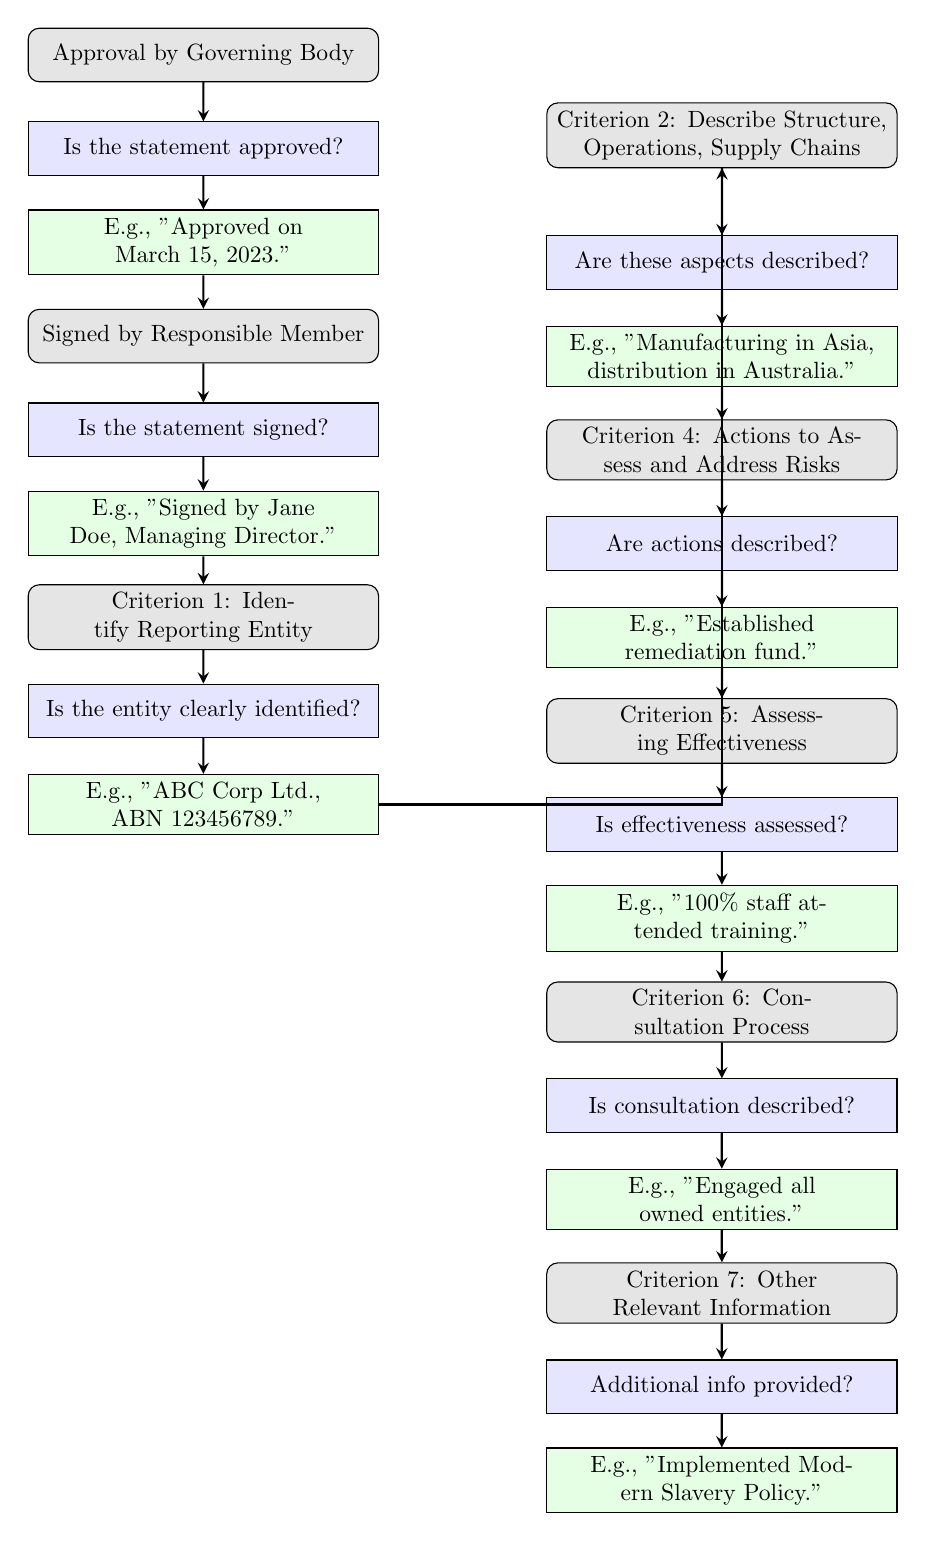
\begin{tikzpicture}[node distance=1.4cm, every node/.style={align=left}, scale=0.85, transform shape]

% Define the styles
\tikzstyle{criterion} = [rectangle, rounded corners, minimum width=5cm, text width=5cm, minimum height=0.8cm, text centered, draw=black, fill=gray!20]
\tikzstyle{question} = [rectangle, minimum width=5cm, text width=5cm, minimum height=0.8cm, text centered, draw=black, fill=blue!10]
\tikzstyle{example} = [rectangle, minimum width=5cm, text width=5cm, minimum height=0.8cm, text centered, draw=black, fill=green!10]
\tikzstyle{arrow} = [thick,->,>=stealth]

% Nodes
\node (C1) [criterion] {Approval by Governing Body};
\node (Q1) [question, below of=C1] {Is the statement approved?};
\node (E1) [example, below of=Q1] {E.g., "Approved on March 15, 2023."};

\node (C2) [criterion, below of=E1] {Signed by Responsible Member};
\node (Q2) [question, below of=C2] {Is the statement signed?};
\node (E2) [example, below of=Q2] {E.g., "Signed by Jane Doe, Managing Director."};

\node (C3) [criterion, below of=E2] {Criterion 1: Identify Reporting Entity};
\node (Q3) [question, below of=C3] {Is the entity clearly identified?};
\node (E3) [example, below of=Q3] {E.g., "ABC Corp Ltd., ABN 123456789."};

\node (C4) [criterion, right=2.5cm of C1, yshift=-1.2cm] {Criterion 2: Describe Structure, Operations, Supply Chains};
\node (Q4) [question, below of=C4, yshift=-0.5cm] {Are these aspects described?};
\node (E4) [example, below of=Q4] {E.g., "Manufacturing in Asia, distribution in Australia."};

\node (C5) [criterion, below of=E4] {Criterion 4: Actions to Assess and Address Risks};
\node (Q5) [question, below of=C5] {Are actions described?};
\node (E5) [example, below of=Q5] {E.g., "Established remediation fund."};

\node (C6) [criterion, below of=E5] {Criterion 5: Assessing Effectiveness};
\node (Q6) [question, below of=C6] {Is effectiveness assessed?};
\node (E6) [example, below of=Q6] {E.g., "100\% staff attended training."};

\node (C7) [criterion, below of=E6] {Criterion 6: Consultation Process};
\node (Q7) [question, below of=C7] {Is consultation described?};
\node (E7) [example, below of=Q7] {E.g., "Engaged all owned entities."};

\node (C8) [criterion, below of=E7] {Criterion 7: Other Relevant Information};
\node (Q8) [question, below of=C8] {Additional info provided?};
\node (E8) [example, below of=Q8] {E.g., "Implemented Modern Slavery Policy."};

% Draw arrows
\draw [arrow] (C1) -- (Q1);
\draw [arrow] (Q1) -- (E1);
\draw [arrow] (E1) -- (C2);
\draw [arrow] (C2) -- (Q2);
\draw [arrow] (Q2) -- (E2);
\draw [arrow] (E2) -- (C3);
\draw [arrow] (C3) -- (Q3);
\draw [arrow] (Q3) -- (E3);

\draw [arrow] (E3) -| (C4);
\draw [arrow] (C4) -- (Q4);
\draw [arrow] (Q4) -- (E4);
\draw [arrow] (E4) -- (C5);
\draw [arrow] (C5) -- (Q5);
\draw [arrow] (Q5) -- (E5);
\draw [arrow] (E5) -- (C6);
\draw [arrow] (C6) -- (Q6);
\draw [arrow] (Q6) -- (E6);
\draw [arrow] (E6) -- (C7);
\draw [arrow] (C7) -- (Q7);
\draw [arrow] (Q7) -- (E7);
\draw [arrow] (E7) -- (C8);
\draw [arrow] (C8) -- (Q8);
\draw [arrow] (Q8) -- (E8);

\end{tikzpicture}
\caption{Flowchart of Mandatory Reporting Criteria under the Australian Modern Slavery Act}
\label{fig:modern_slavery_flowchart}
\end{figure}






\begin{figure}[ht]
    \centering
    \caption{Illustration of Australian Modern Slavery Act Mandatory Reporting Criteria}
    \label{fig:modern_slavery_illustration}
    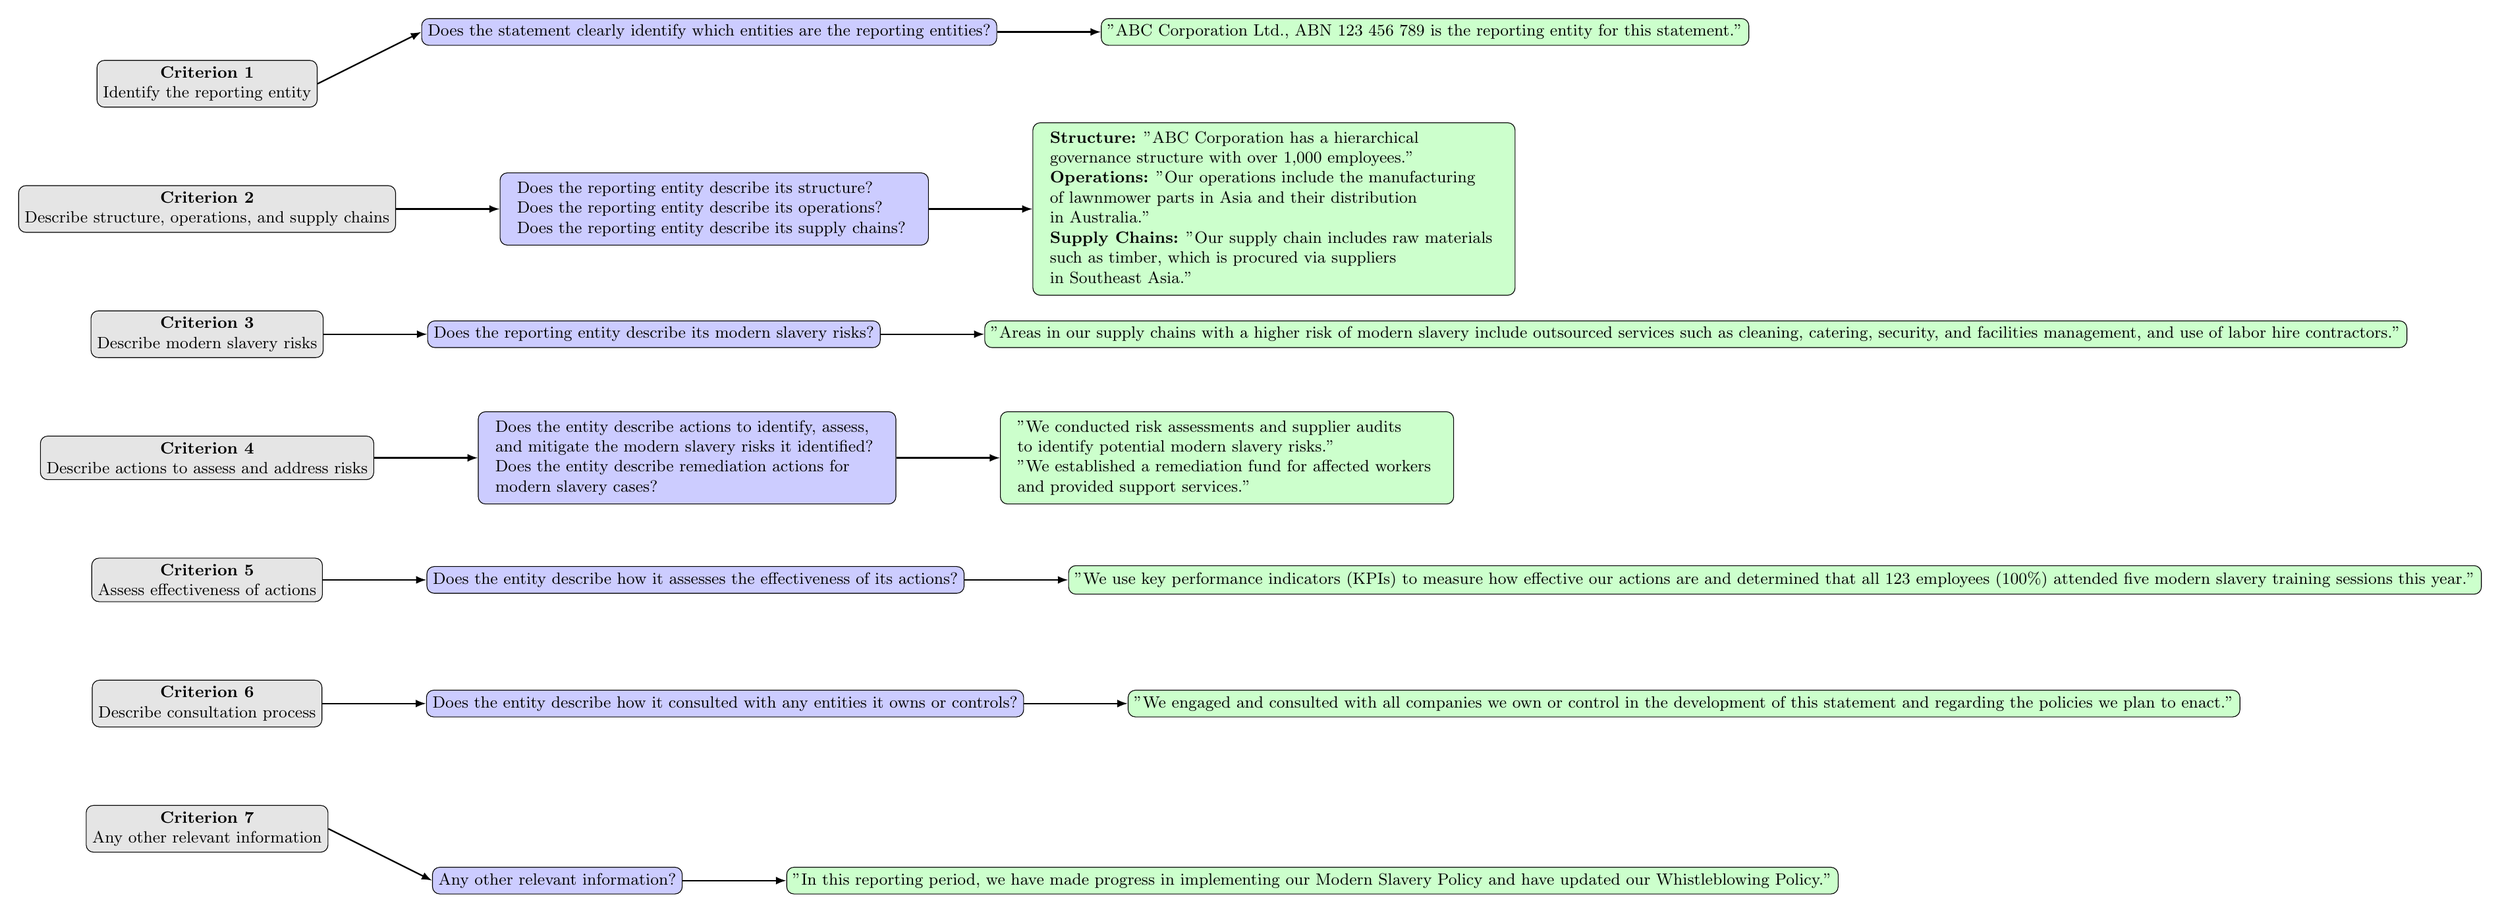
\begin{tikzpicture}[
        node distance=1.5cm and 2cm,
        every node/.style={rectangle, draw=black, rounded corners, align=center, minimum width=4cm, font=\small},
        criterion/.style={fill=gray!20},
        question/.style={fill=blue!20},
        example/.style={fill=green!20},
        arrow/.style={-{Latex[length=2mm]}, thick}
    ]
    % Nodes for Mandatory Criteria
    \node[criterion] (criterion1) {\textbf{Criterion 1}\\Identify the reporting entity};
    \node[criterion, below=of criterion1] (criterion2) {\textbf{Criterion 2}\\Describe structure, operations, and supply chains};
    \node[criterion, below=of criterion2] (criterion3) {\textbf{Criterion 3}\\Describe modern slavery risks};
    \node[criterion, below=of criterion3] (criterion4) {\textbf{Criterion 4}\\Describe actions to assess and address risks};
    \node[criterion, below=of criterion4] (criterion5) {\textbf{Criterion 5}\\Assess effectiveness of actions};
    \node[criterion, below=of criterion5] (criterion6) {\textbf{Criterion 6}\\Describe consultation process};
    \node[criterion, below=of criterion6] (criterion7) {\textbf{Criterion 7}\\Any other relevant information};

    % Questions connected to Criteria
    \node[question, right=of criterion1, yshift=1cm] (question1) {Does the statement clearly identify which entities are the reporting entities?};
    \node[question, right=of criterion2] (question2) {
        \begin{tabular}{l}
            Does the reporting entity describe its structure?\\
            Does the reporting entity describe its operations?\\
            Does the reporting entity describe its supply chains?
        \end{tabular}
    };
    \node[question, right=of criterion3] (question3) {Does the reporting entity describe its modern slavery risks?};
    \node[question, right=of criterion4] (question4) {
        \begin{tabular}{l}
            Does the entity describe actions to identify, assess,\\
            and mitigate the modern slavery risks it identified?\\
            Does the entity describe remediation actions for\\
            modern slavery cases?
        \end{tabular}
    };
    \node[question, right=of criterion5] (question5) {Does the entity describe how it assesses the effectiveness of its actions?};
    \node[question, right=of criterion6] (question6) {Does the entity describe how it consulted with any entities it owns or controls?};
    \node[question, right=of criterion7, yshift=-1cm] (question7) {Any other relevant information?};

    % Examples connected to Questions
    \node[example, right=of question1, yshift=0cm] (example1) {"ABC Corporation Ltd., ABN 123 456 789 is the reporting entity for this statement."};
    \node[example, right=of question2] (example2) {
        \begin{tabular}{l}
            \textbf{Structure:} "ABC Corporation has a hierarchical\\ governance structure with over 1,000 employees."\\
            \textbf{Operations:} "Our operations include the manufacturing\\ of lawnmower parts in Asia and their distribution\\ in Australia."\\
            \textbf{Supply Chains:} "Our supply chain includes raw materials\\ such as timber, which is procured via suppliers\\ in Southeast Asia."
        \end{tabular}
    };
    \node[example, right=of question3] (example3) {"Areas in our supply chains with a higher risk of modern slavery include outsourced services such as cleaning, catering, security, and facilities management, and use of labor hire contractors."};
    \node[example, right=of question4] (example4) {
        \begin{tabular}{l}
            "We conducted risk assessments and supplier audits\\ to identify potential modern slavery risks."\\
            "We established a remediation fund for affected workers\\ and provided support services."
        \end{tabular}
    };
    \node[example, right=of question5] (example5) {"We use key performance indicators (KPIs) to measure how effective our actions are and determined that all 123 employees (100\%) attended five modern slavery training sessions this year."};
    \node[example, right=of question6] (example6) {"We engaged and consulted with all companies we own or control in the development of this statement and regarding the policies we plan to enact."};
    \node[example, right=of question7] (example7) {"In this reporting period, we have made progress in implementing our Modern Slavery Policy and have updated our Whistleblowing Policy."};

    % Draw arrows between nodes
    \draw[arrow] (criterion1.east) -- (question1.west);
    \draw[arrow] (question1.east) -- (example1.west);

    \draw[arrow] (criterion2.east) -- (question2.west);
    \draw[arrow] (question2.east) -- (example2.west);

    \draw[arrow] (criterion3.east) -- (question3.west);
    \draw[arrow] (question3.east) -- (example3.west);

    \draw[arrow] (criterion4.east) -- (question4.west);
    \draw[arrow] (question4.east) -- (example4.west);

    \draw[arrow] (criterion5.east) -- (question5.west);
    \draw[arrow] (question5.east) -- (example5.west);

    \draw[arrow] (criterion6.east) -- (question6.west);
    \draw[arrow] (question6.east) -- (example6.west);

    \draw[arrow] (criterion7.east) -- (question7.west);
    \draw[arrow] (question7.east) -- (example7.west);
    \end{tikzpicture}
\end{figure}


\documentclass{article}
\usepackage[utf8]{inputenc}
\usepackage{tikz}
\usetikzlibrary{shapes, arrows.meta, positioning, fit}
\usepackage{geometry}
\geometry{a4paper, margin=1in}


\begin{figure}[ht]
    \centering
    \caption{Illustration of Australian Modern Slavery Act Mandatory Reporting Criteria}
    \label{fig:modern_slavery_illustration}
    \resizebox{\textwidth}{!}{
    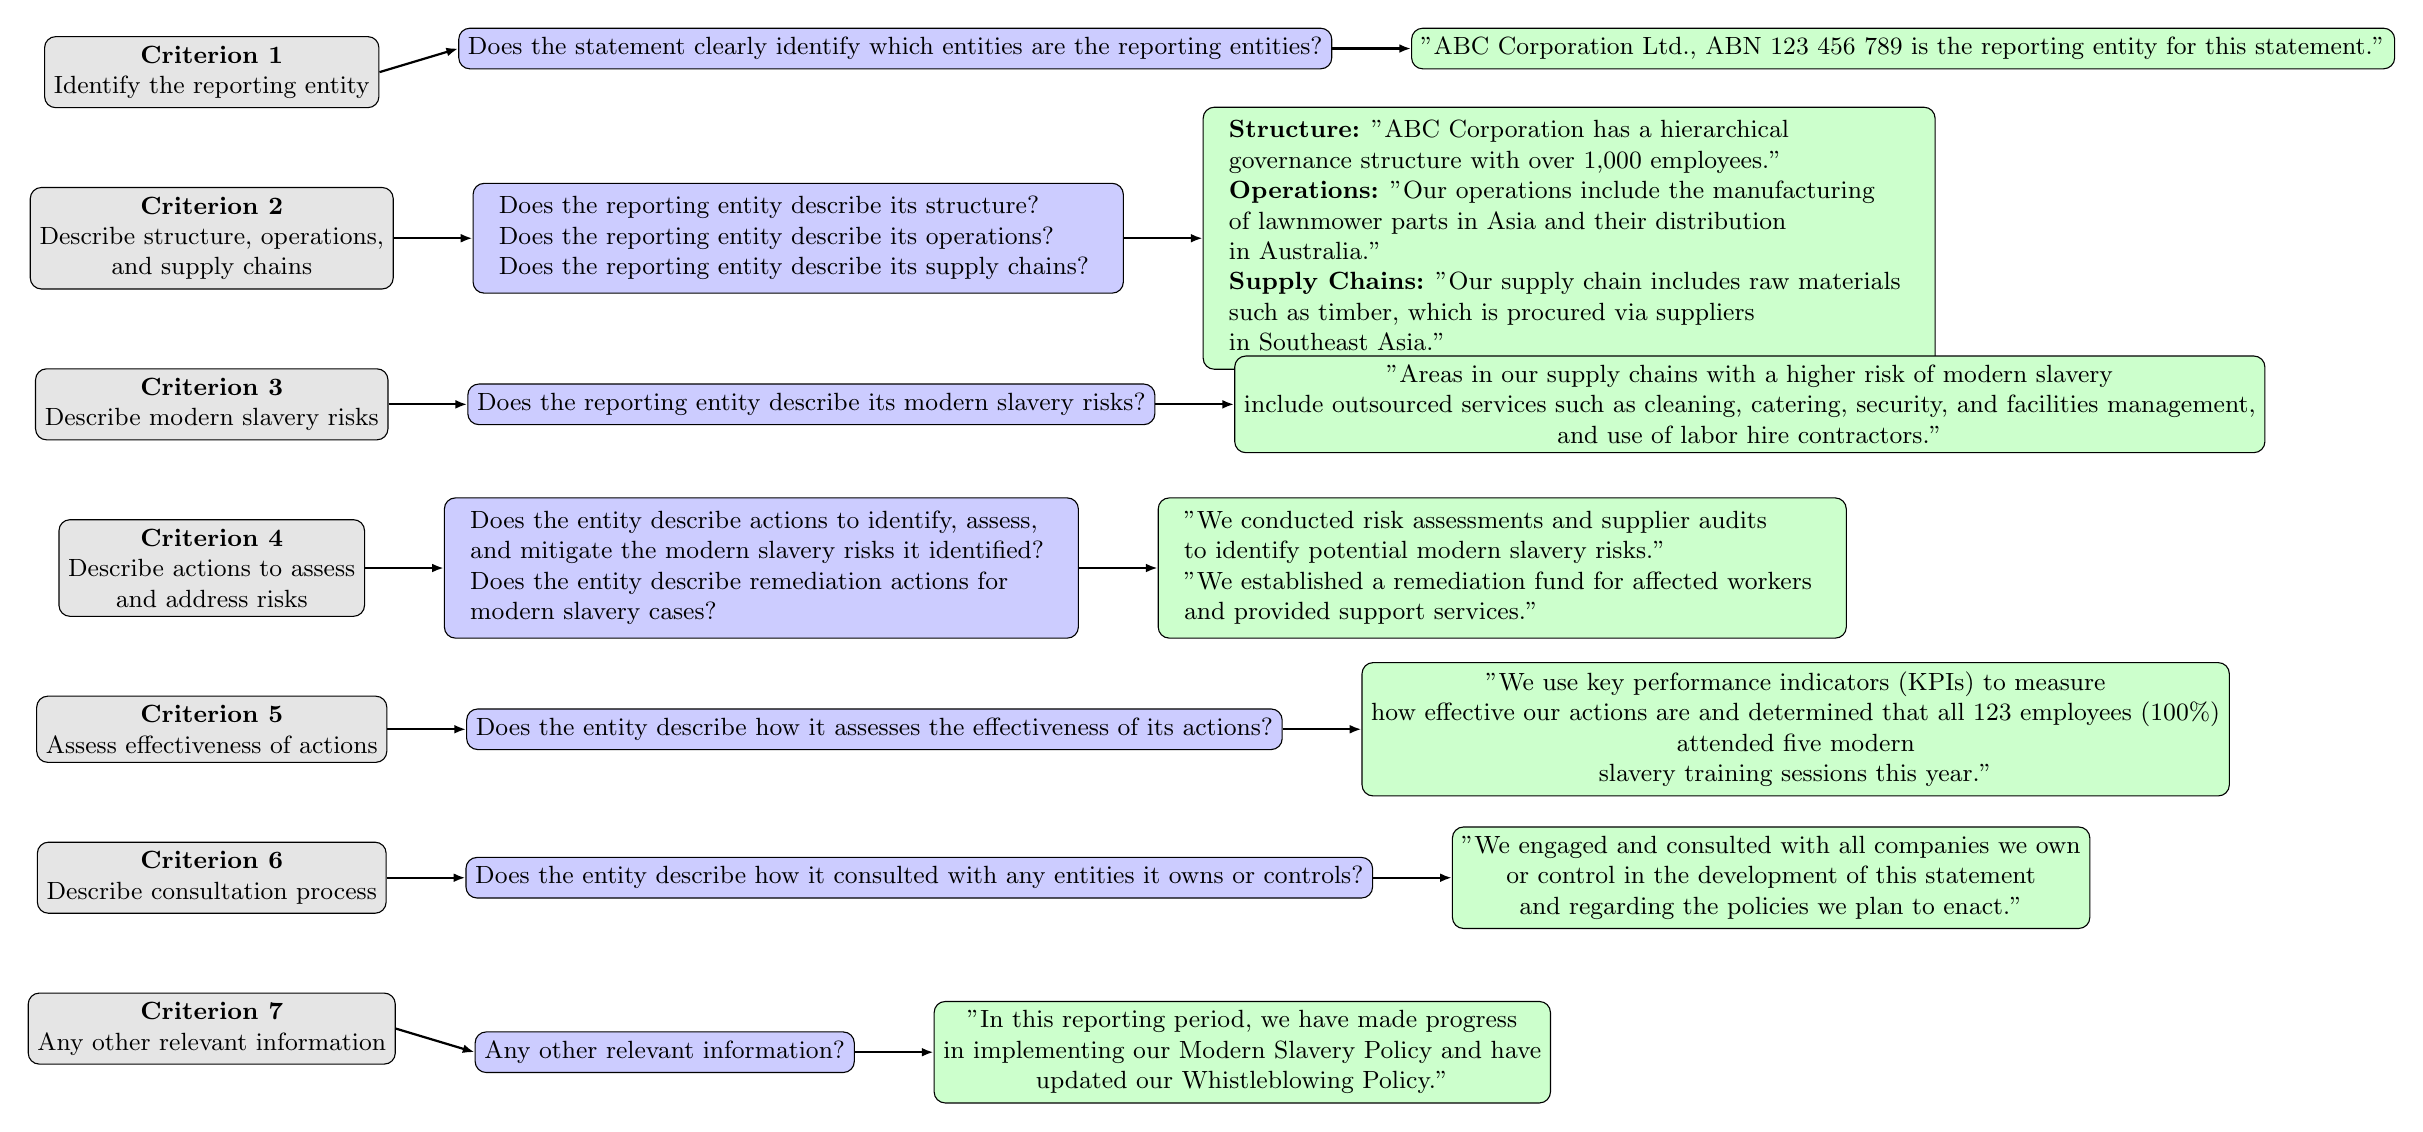
\begin{tikzpicture}[
        node distance= 1cm and 1cm,
        every node/.style={rectangle, draw=black, rounded corners, align=center, minimum width=2.5cm, font=\small},
        criterion/.style={fill=gray!20},
        question/.style={fill=blue!20},
        example/.style={fill=green!20},
        arrow/.style={-{Latex[length=1.5mm]}, thick}
    ]
    % Nodes for Mandatory Criteria
    \node[criterion] (criterion1) {\textbf{Criterion 1}\\Identify the reporting entity};
    \node[criterion, below=of criterion1] (criterion2) {\textbf{Criterion 2}\\Describe structure, operations,\\and supply chains};
    \node[criterion, below=of criterion2] (criterion3) {\textbf{Criterion 3}\\Describe modern slavery risks};
    \node[criterion, below=of criterion3] (criterion4) {\textbf{Criterion 4}\\Describe actions to assess\\and address risks};
    \node[criterion, below=of criterion4] (criterion5) {\textbf{Criterion 5}\\Assess effectiveness of actions};
    \node[criterion, below=of criterion5] (criterion6) {\textbf{Criterion 6}\\Describe consultation process};
    \node[criterion, below=of criterion6] (criterion7) {\textbf{Criterion 7}\\Any other relevant information};

    % Questions connected to Criteria
    \node[question, right=of criterion1, yshift=0.3cm] (question1) {Does the statement clearly identify which entities are the reporting entities?};
    \node[question, right=of criterion2] (question2) {
        \begin{tabular}{l}
            Does the reporting entity describe its structure?\\
            Does the reporting entity describe its operations?\\
            Does the reporting entity describe its supply chains?
        \end{tabular}
    };
    \node[question, right=of criterion3] (question3) {Does the reporting entity describe its modern slavery risks?};
    \node[question, right=of criterion4] (question4) {
        \begin{tabular}{l}
            Does the entity describe actions to identify, assess,\\
            and mitigate the modern slavery risks it identified?\\
            Does the entity describe remediation actions for\\
            modern slavery cases?
        \end{tabular}
    };
    \node[question, right=of criterion5] (question5) {Does the entity describe how it assesses the effectiveness of its actions?};
    \node[question, right=of criterion6] (question6) {Does the entity describe how it consulted with any entities it owns or controls?};
    \node[question, right=of criterion7, yshift=-0.3cm] (question7) {Any other relevant information?};

    % Examples connected to Questions
    \node[example, right=of question1, yshift=0cm] (example1) {"ABC Corporation Ltd., ABN 123 456 789 is the reporting entity for this statement."};
    \node[example, right=of question2] (example2) {
        \begin{tabular}{l}
            \textbf{Structure:} "ABC Corporation has a hierarchical\\governance structure with over 1,000 employees."\\
            \textbf{Operations:} "Our operations include the manufacturing\\of lawnmower parts in Asia and their distribution\\in Australia."\\
            \textbf{Supply Chains:} "Our supply chain includes raw materials\\such as timber, which is procured via suppliers\\in Southeast Asia."
        \end{tabular}
    };
    \node[example, right=of question3] (example3) {"Areas in our supply chains with a higher risk of modern slavery \\
    include outsourced services such as cleaning, catering, security, and facilities management, \\
    and use of labor hire contractors."};
    \node[example, right=of question4] (example4) {
        \begin{tabular}{l}
            "We conducted risk assessments and supplier audits\\to identify potential modern slavery risks."\\
            "We established a remediation fund for affected workers\\and provided support services."
        \end{tabular}
    };
    \node[example, right=of question5] (example5) {"We use key performance indicators (KPIs) to measure \\
    how effective our actions are and determined that all 123 employees (100\%)\\
    attended five modern \\
    slavery training sessions this year."};
    \node[example, right=of question6] (example6) {"We engaged and consulted with all companies we own\\
    or control in the development of this statement \\
    and regarding the policies we plan to enact."};
    \node[example, right=of question7] (example7) {"In this reporting period, we have made progress \\
    in implementing our Modern Slavery Policy and have \\
    updated our Whistleblowing Policy."};

    % Draw arrows between nodes
    \draw[arrow] (criterion1.east) -- (question1.west);
    \draw[arrow] (question1.east) -- (example1.west);

    \draw[arrow] (criterion2.east) -- (question2.west);
    \draw[arrow] (question2.east) -- (example2.west);

    \draw[arrow] (criterion3.east) -- (question3.west);
    \draw[arrow] (question3.east) -- (example3.west);

    \draw[arrow] (criterion4.east) -- (question4.west);
    \draw[arrow] (question4.east) -- (example4.west);

    \draw[arrow] (criterion5.east) -- (question5.west);
    \draw[arrow] (question5.east) -- (example5.west);

    \draw[arrow] (criterion6.east) -- (question6.west);
    \draw[arrow] (question6.east) -- (example6.west);

    \draw[arrow] (criterion7.east) -- (question7.west);
    \draw[arrow] (question7.east) -- (example7.west);
    \end{tikzpicture}
    }
\end{figure}


\documentclass{article}
\usepackage[utf8]{inputenc}
\usepackage{tikz}
\usetikzlibrary{shapes, arrows.meta, positioning, fit}
\usepackage{geometry}
\geometry{a4paper, margin=1in}

\begin{document}

\begin{figure}[ht]
    \centering
    \caption{Illustration of Australian Modern Slavery Act Mandatory Reporting Criteria}
    \label{fig:modern_slavery_illustration}
    \resizebox{\textwidth}{!}{
    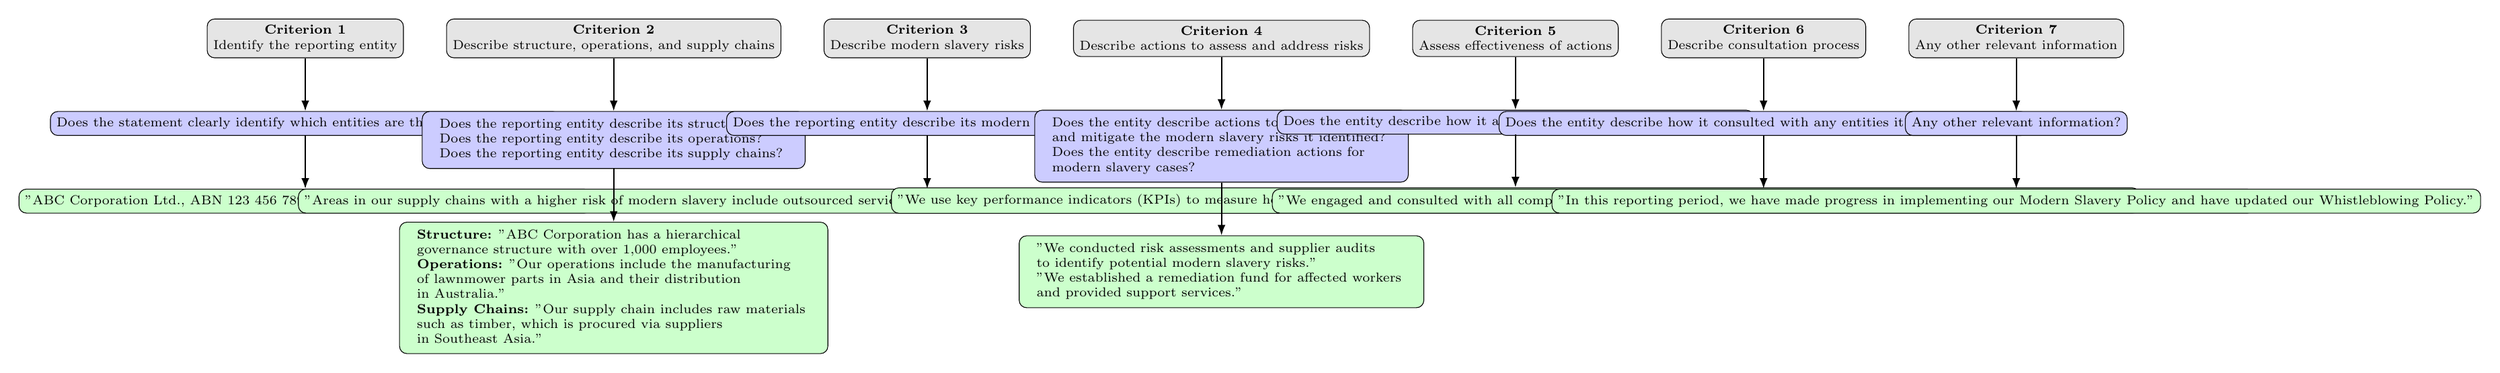
\begin{tikzpicture}[
        node distance=1cm and 0.8cm,
        every node/.style={rectangle, draw=black, rounded corners, align=center, minimum width=3cm, font=\scriptsize},
        criterion/.style={fill=gray!20},
        question/.style={fill=blue!20},
        example/.style={fill=green!20},
        arrow/.style={-{Latex[length=2mm]}, thick}
    ]
    % First Row: Criteria
    \node[criterion] (criterion1) {\textbf{Criterion 1}\\Identify the reporting entity};
    \node[criterion, right=of criterion1] (criterion2) {\textbf{Criterion 2}\\Describe structure, operations, and supply chains};
    \node[criterion, right=of criterion2] (criterion3) {\textbf{Criterion 3}\\Describe modern slavery risks};
    \node[criterion, right=of criterion3] (criterion4) {\textbf{Criterion 4}\\Describe actions to assess and address risks};
    \node[criterion, right=of criterion4] (criterion5) {\textbf{Criterion 5}\\Assess effectiveness of actions};
    \node[criterion, right=of criterion5] (criterion6) {\textbf{Criterion 6}\\Describe consultation process};
    \node[criterion, right=of criterion6] (criterion7) {\textbf{Criterion 7}\\Any other relevant information};

    % Second Row: Questions
    \node[question, below=of criterion1] (question1) {Does the statement clearly identify which entities are the reporting entities?};
    \node[question, below=of criterion2] (question2) {
        \begin{tabular}{l}
            Does the reporting entity describe its structure?\\
            Does the reporting entity describe its operations?\\
            Does the reporting entity describe its supply chains?
        \end{tabular}
    };
    \node[question, below=of criterion3] (question3) {Does the reporting entity describe its modern slavery risks?};
    \node[question, below=of criterion4] (question4) {
        \begin{tabular}{l}
            Does the entity describe actions to identify, assess,\\
            and mitigate the modern slavery risks it identified?\\
            Does the entity describe remediation actions for\\
            modern slavery cases?
        \end{tabular}
    };
    \node[question, below=of criterion5] (question5) {Does the entity describe how it assesses the effectiveness of its actions?};
    \node[question, below=of criterion6] (question6) {Does the entity describe how it consulted with any entities it owns or controls?};
    \node[question, below=of criterion7] (question7) {Any other relevant information?};

    % Third Row: Examples
    \node[example, below=of question1] (example1) {"ABC Corporation Ltd., ABN 123 456 789 is the reporting entity for this statement."};
    \node[example, below=of question2] (example2) {
        \begin{tabular}{l}
            \textbf{Structure:} "ABC Corporation has a hierarchical\\governance structure with over 1,000 employees."\\
            \textbf{Operations:} "Our operations include the manufacturing\\of lawnmower parts in Asia and their distribution\\in Australia."\\
            \textbf{Supply Chains:} "Our supply chain includes raw materials\\such as timber, which is procured via suppliers\\in Southeast Asia."
        \end{tabular}
    };
    \node[example, below=of question3] (example3) {"Areas in our supply chains with a higher risk of modern slavery include outsourced services such as cleaning, catering, security, and facilities management, and use of labor hire contractors."};
    \node[example, below=of question4] (example4) {
        \begin{tabular}{l}
            "We conducted risk assessments and supplier audits\\to identify potential modern slavery risks."\\
            "We established a remediation fund for affected workers\\and provided support services."
        \end{tabular}
    };
    \node[example, below=of question5] (example5) {"We use key performance indicators (KPIs) to measure how effective our actions are and determined that all 123 employees (100\%) attended five modern slavery training sessions this year."};
    \node[example, below=of question6] (example6) {"We engaged and consulted with all companies we own or control in the development of this statement and regarding the policies we plan to enact."};
    \node[example, below=of question7] (example7) {"In this reporting period, we have made progress in implementing our Modern Slavery Policy and have updated our Whistleblowing Policy."};

    % Arrows from Criteria to Questions
    \foreach \i in {1,...,7}{
        \draw[arrow] (criterion\i.south) -- (question\i.north);
        \draw[arrow] (question\i.south) -- (example\i.north);
    }

    \end{tikzpicture}
    }
\end{figure}

\end{document}


\end{document}
